\begin{frame}[shrink=1]{Visualization of Controllable Generated vs. Natural Proteins}
	\begin{center}
		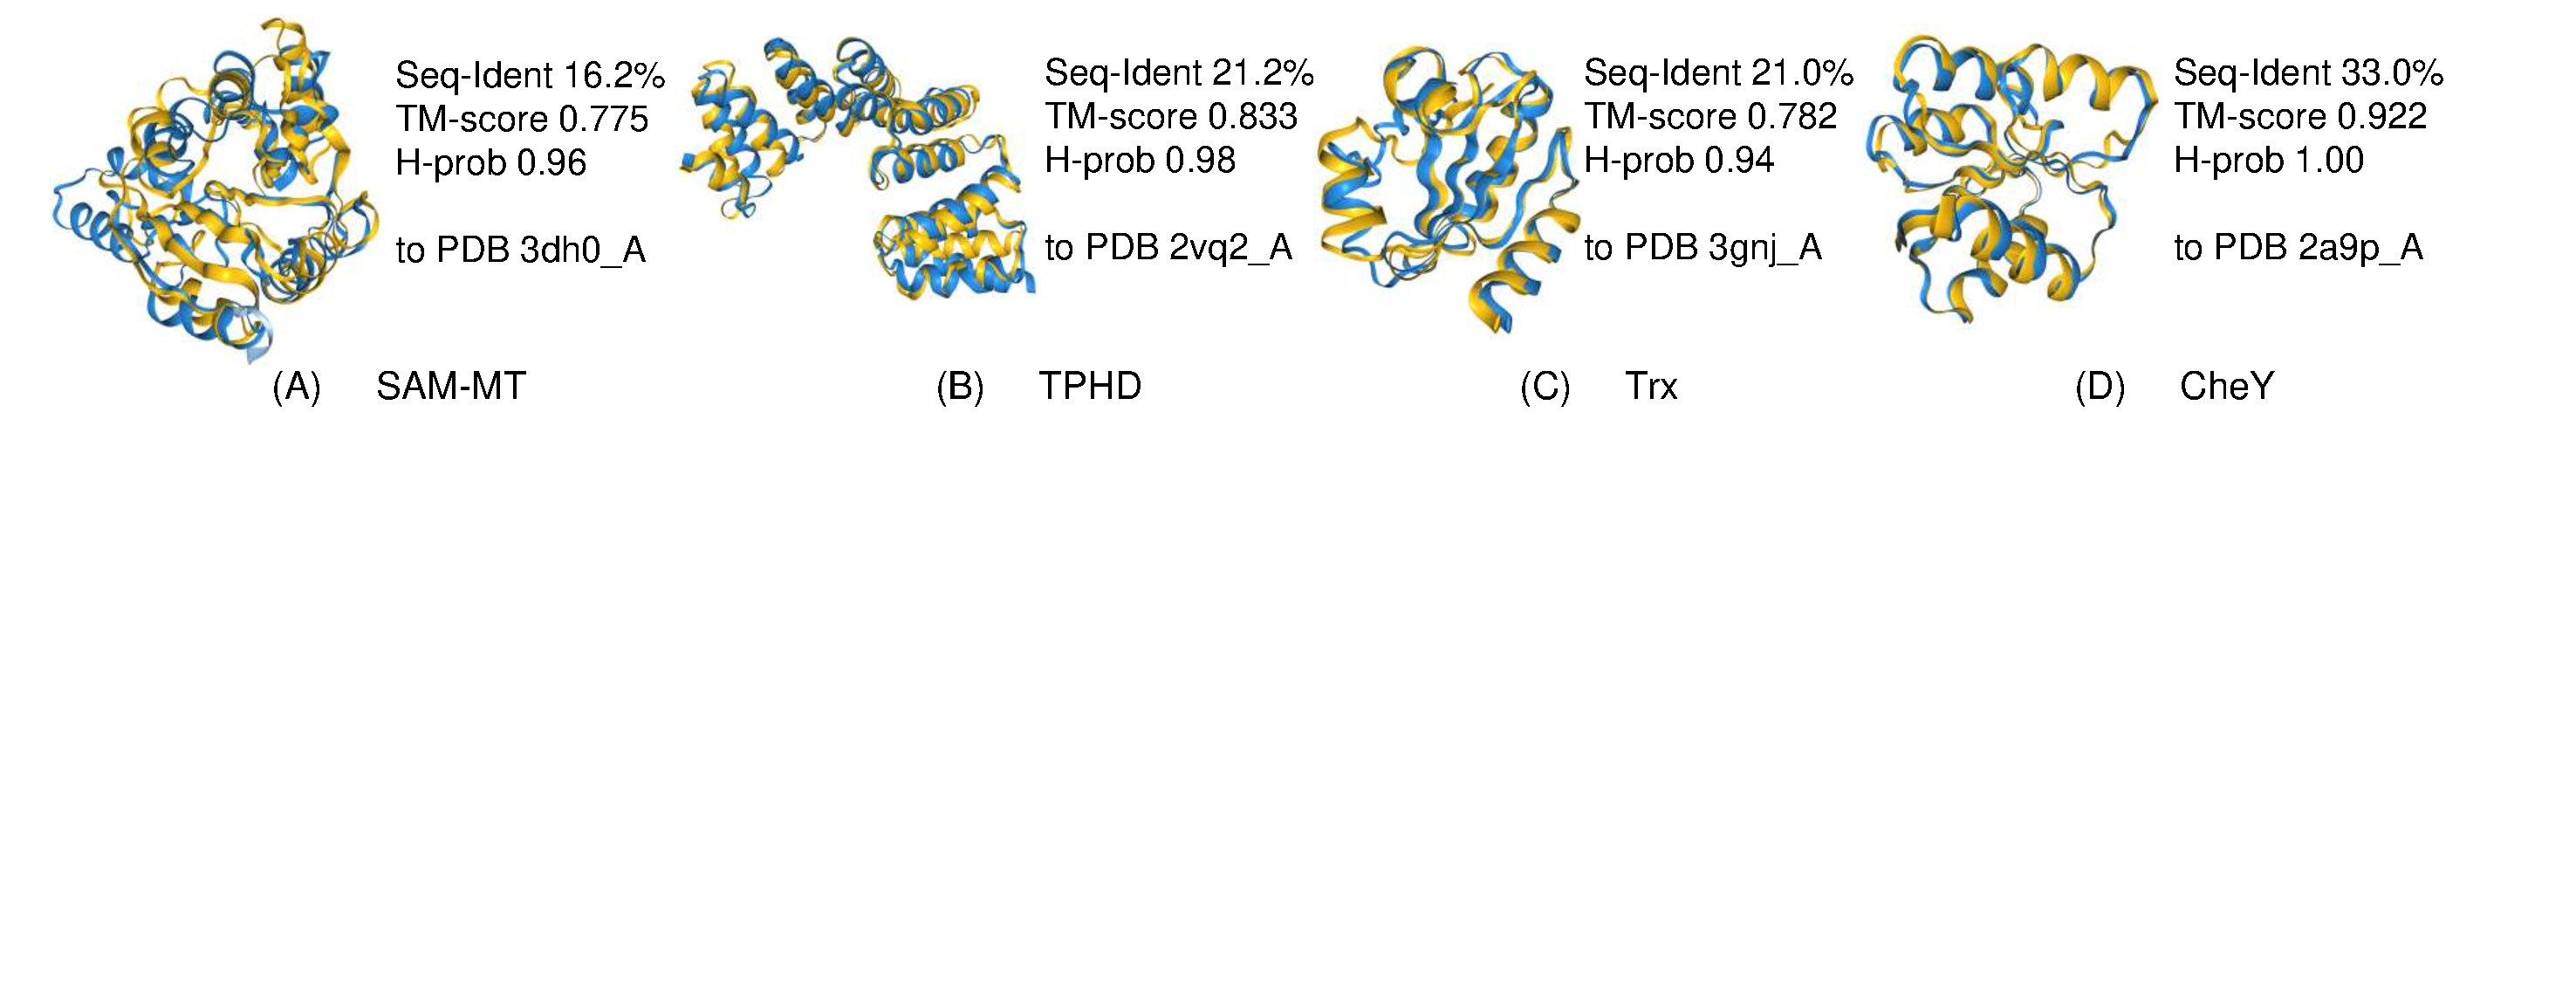
\includegraphics[trim={0 0 90em 0},clip,scale=0.4]{images/protein_visualization.pdf}
		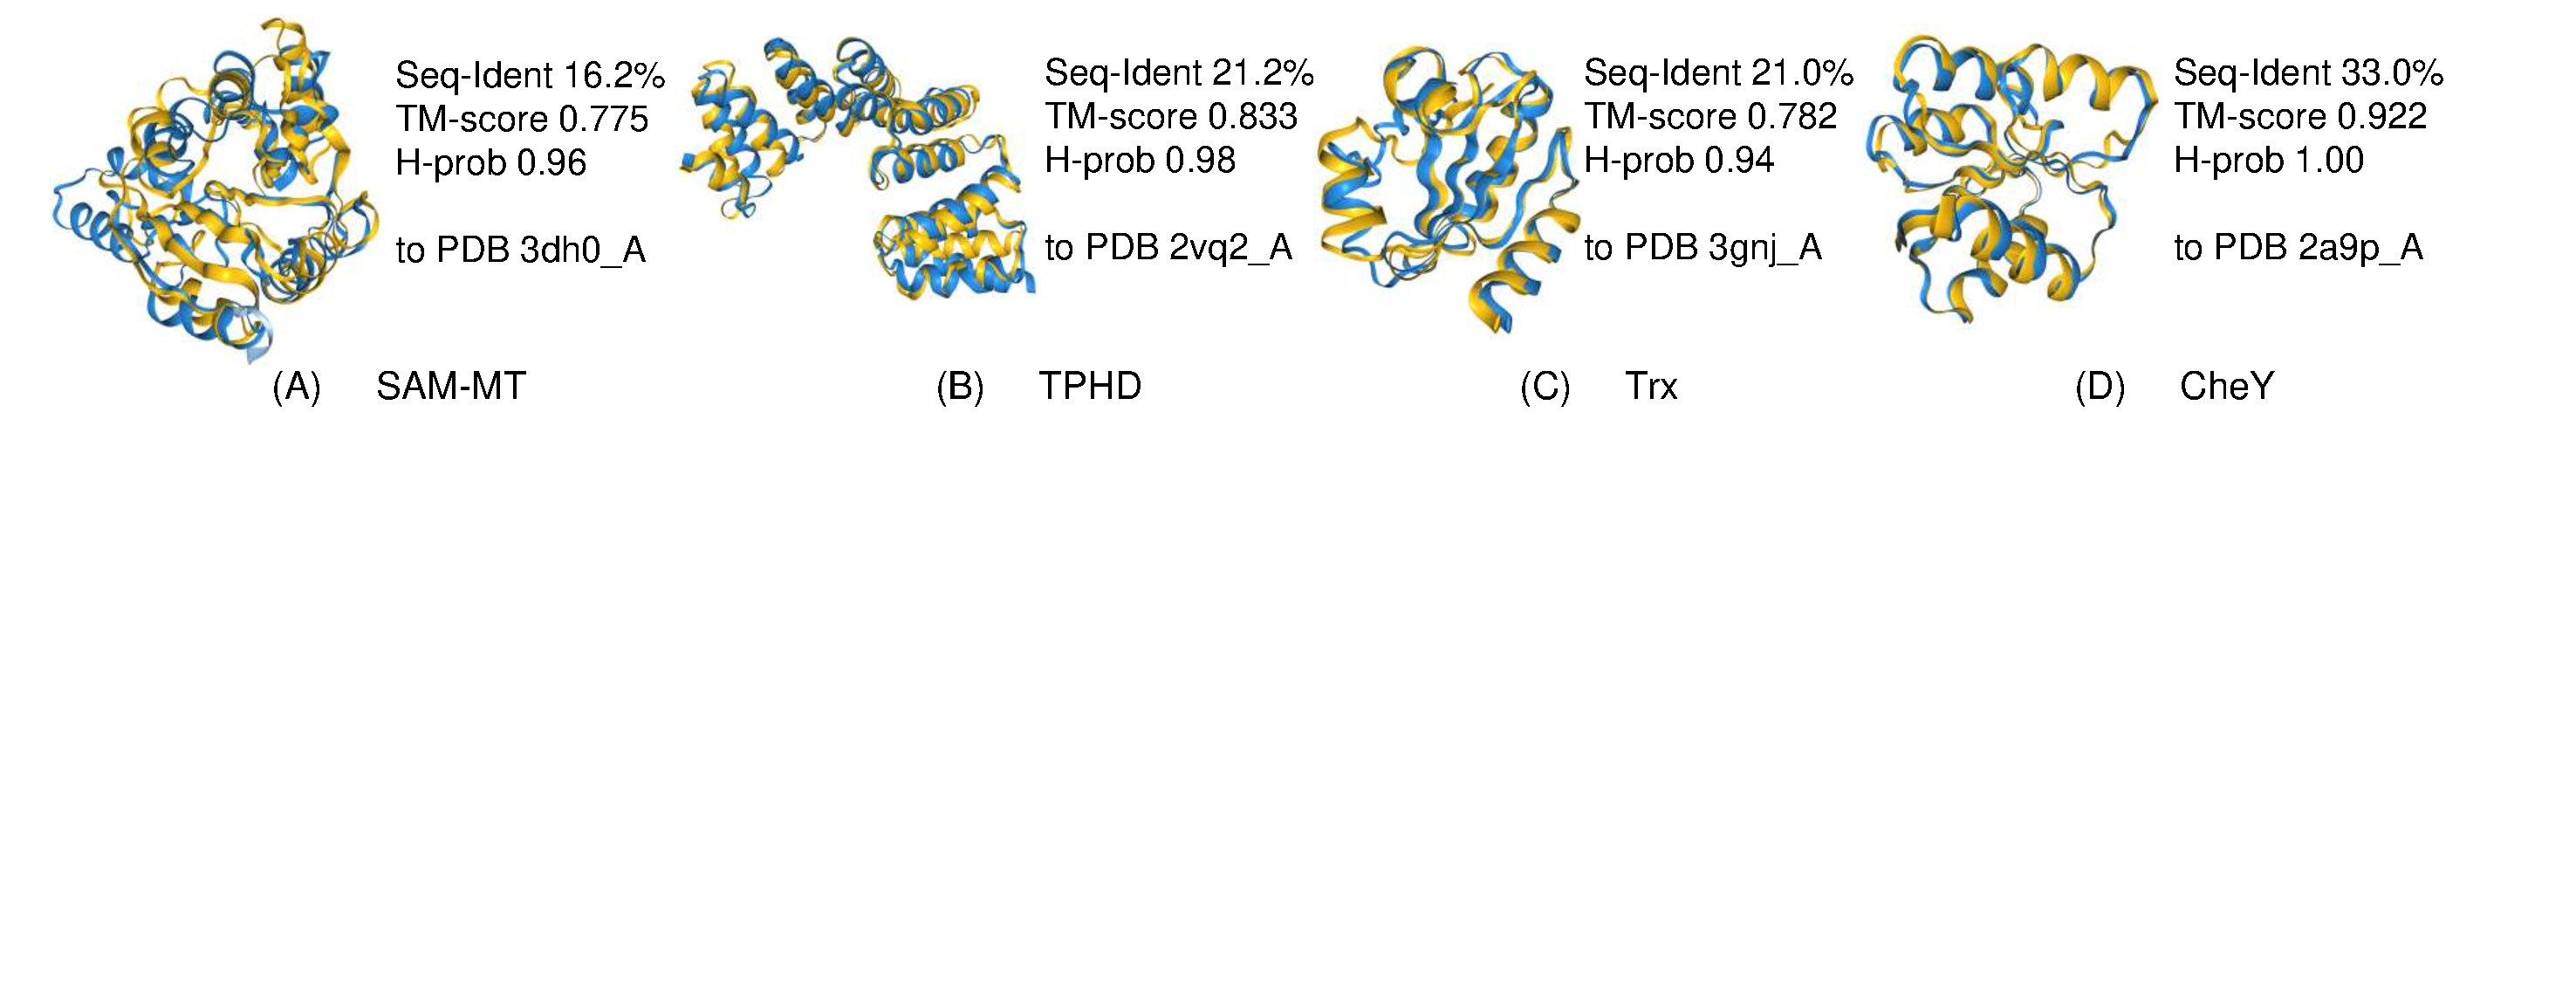
\includegraphics[trim={31.5em 0 57.4em 0},clip,scale=0.4]{images/protein_visualization.pdf}
		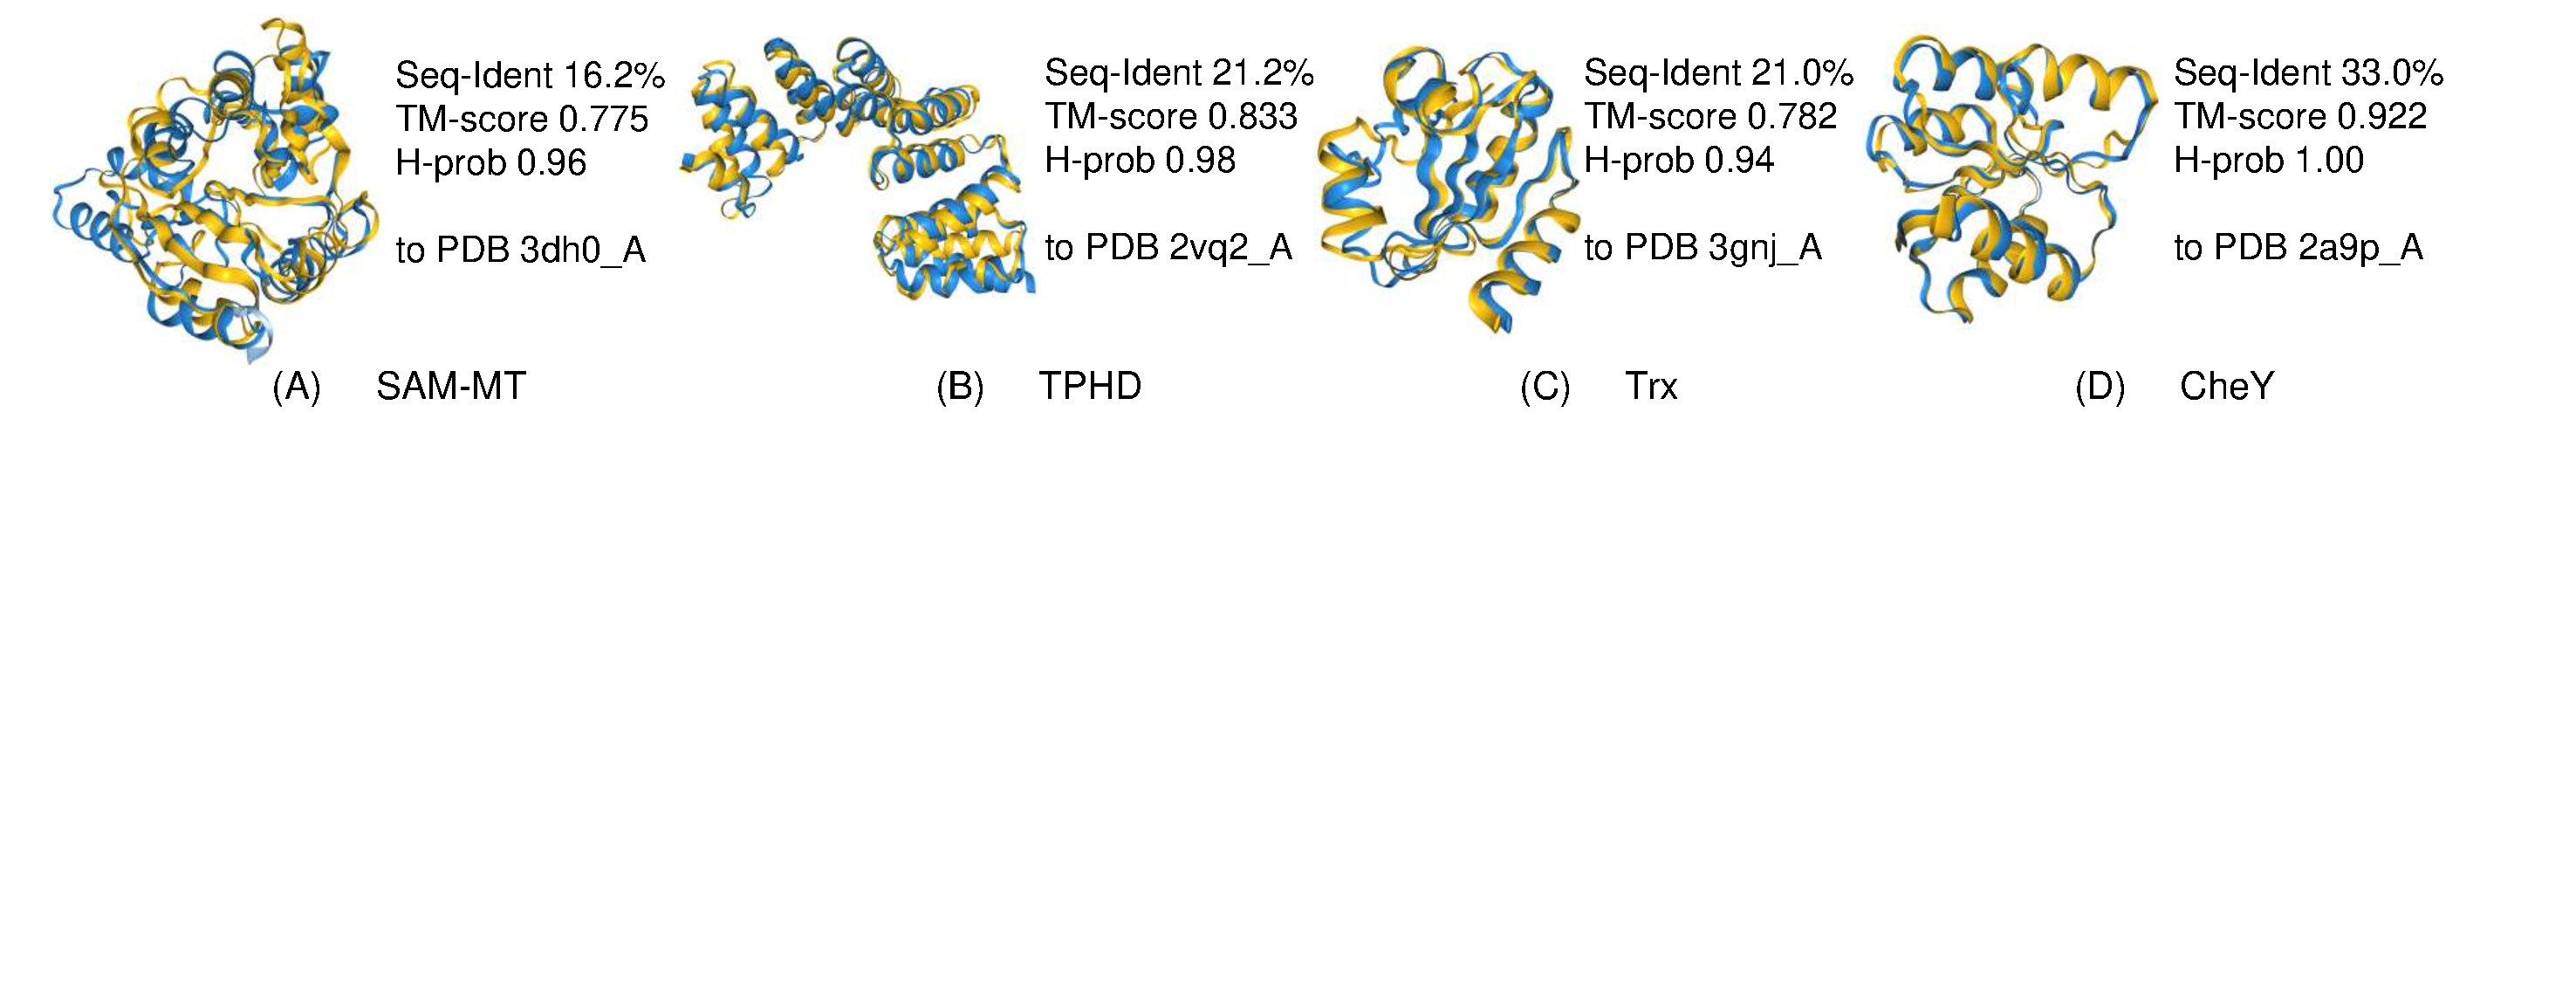
\includegraphics[trim={64em 0 30em 0},clip,scale=0.4]{images/protein_visualization.pdf}
		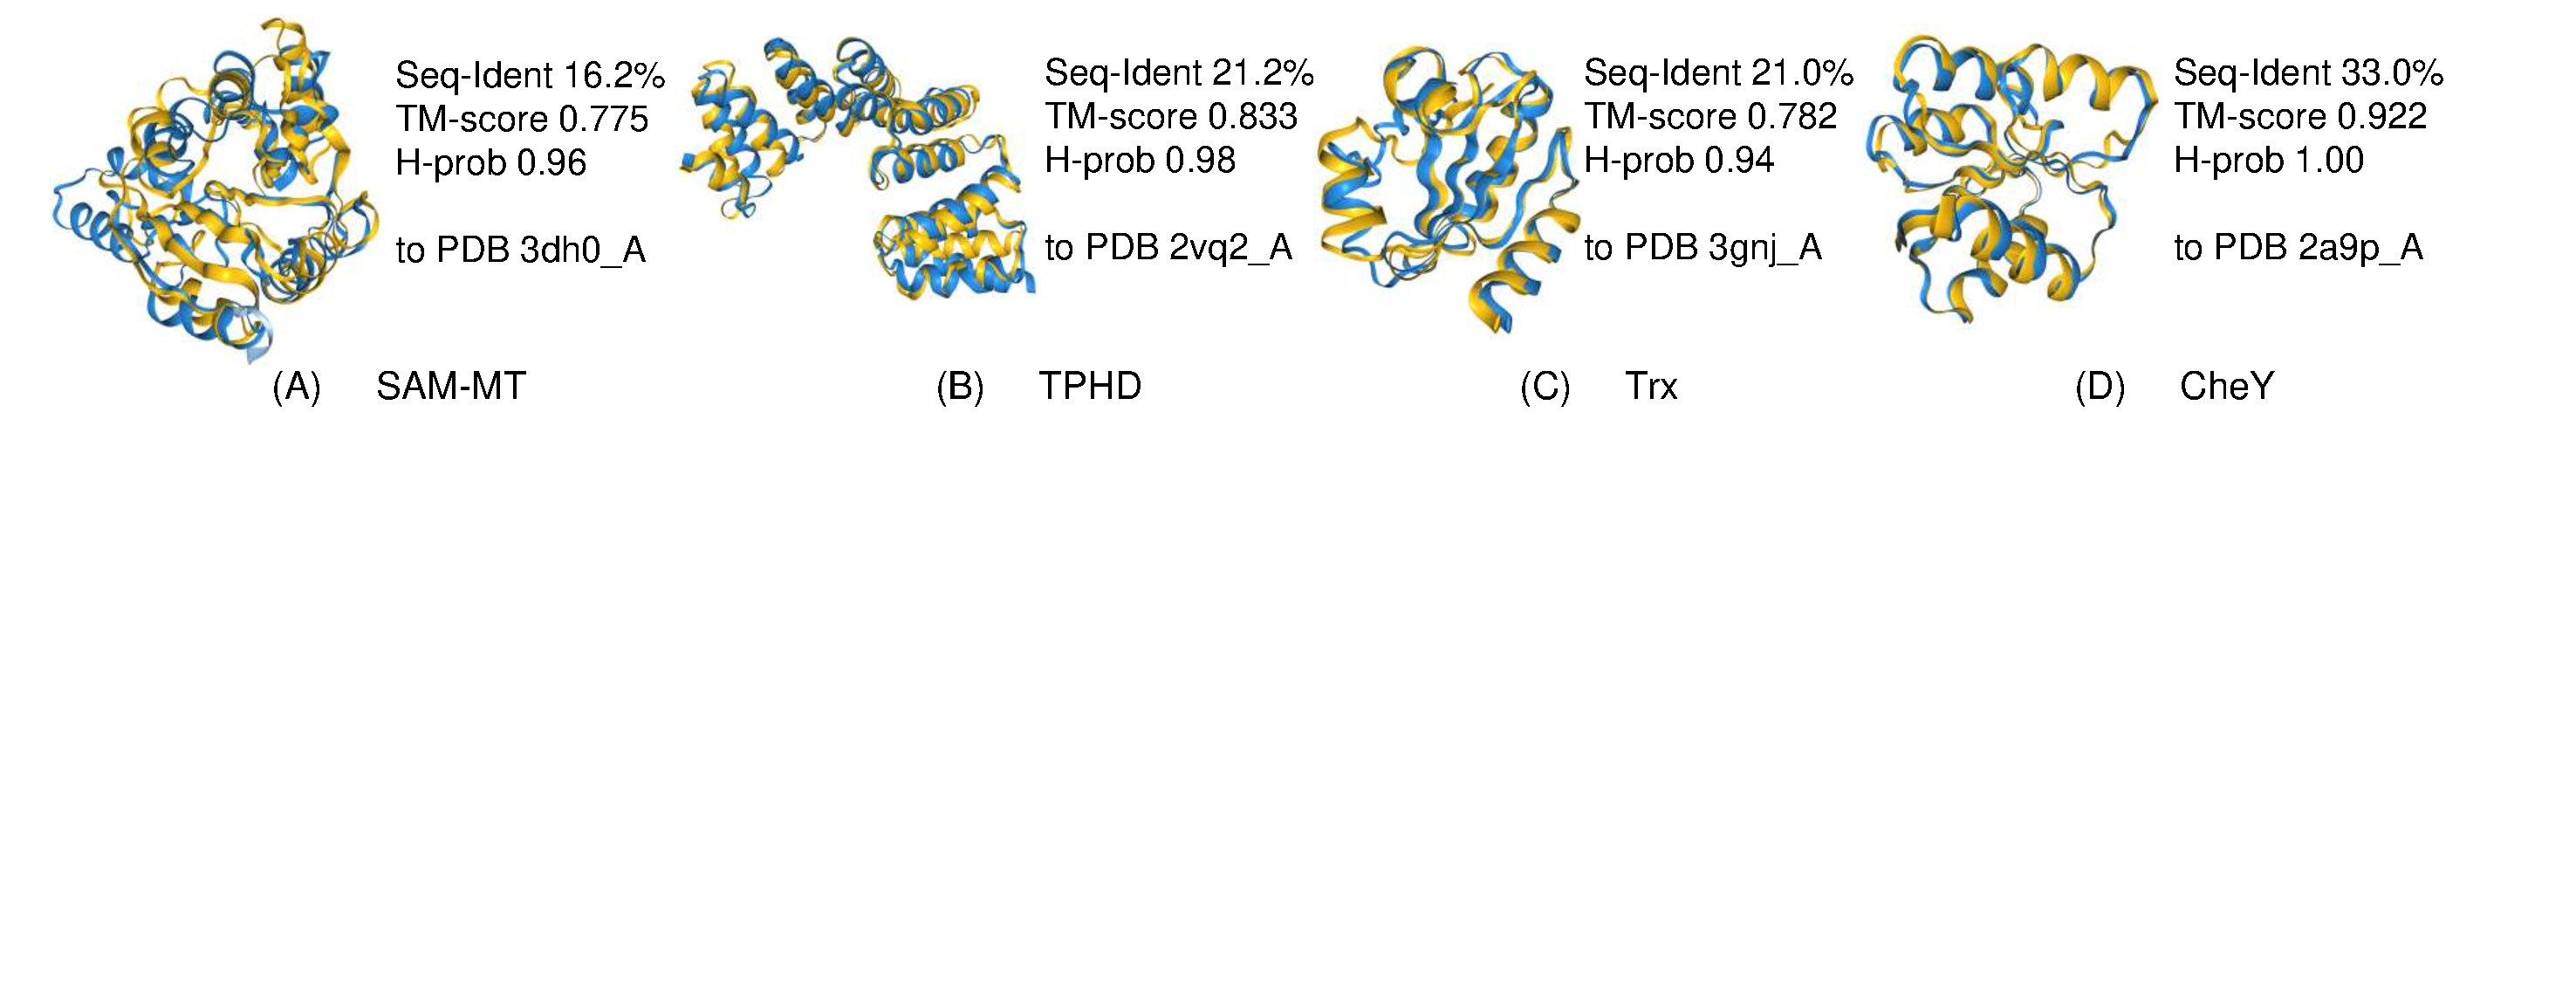
\includegraphics[trim={92em 0 0 0},clip,scale=0.4]{images/protein_visualization.pdf}
	\end{center}
	\vspace{-1em}\credit{Image}{lv2024prollama}
	\begin{itemize}
		\item Blue: generated proteins by superfamily, yellow: the most structurally similar natural proteins (counterparts) from PDB
		\item Generated and natural proteins belong to the same superfamily (source: InterPro)
		\item Similar in structure (function), different in sequence (novel)
	\end{itemize}
\end{frame}